\documentclass[14pt]{extbook}
\usepackage{multicol, enumerate, enumitem, hyperref, color, soul, setspace, parskip, fancyhdr} %General Packages
\usepackage{amssymb, amsthm, amsmath, bbm, latexsym, units, mathtools} %Math Packages
\everymath{\displaystyle} %All math in Display Style
% Packages with additional options
\usepackage[headsep=0.5cm,headheight=12pt, left=1 in,right= 1 in,top= 1 in,bottom= 1 in]{geometry}
\usepackage[usenames,dvipsnames]{xcolor}
\usepackage{dashrule}  % Package to use the command below to create lines between items
\newcommand{\litem}[1]{\item#1\hspace*{-1cm}\rule{\textwidth}{0.4pt}}
\pagestyle{fancy}
\lhead{Makeup Progress Quiz 3}
\chead{}
\rhead{Version B}
\lfoot{4315-3397}
\cfoot{}
\rfoot{Fall 2020}
\begin{document}

\begin{enumerate}
\litem{
Determine the vertical asymptotes and holes in the rational function below.\[ f(x) = \frac{8x^{3} -26 x^{2} -5 x + 50}{8x^{2} +22 x + 15} \]\begin{enumerate}[label=\Alph*.]
\item \( \text{Holes at } x = -1.5 \text{ and } x = -1.25 \text{ with no vertical asymptotes.} \)
\item \( \text{Vertical Asymptotes of } x = -1.5 \text{ and } x = -1.25 \text{ with no holes.} \)
\item \( \text{Vertical Asymptotes of } x = -1.5 \text{ and } x = 2.5 \text{ with a hole at } x = -1.25 \)
\item \( \text{Vertical Asymptote of } x = -1.5 \text{ and hole at } x = -1.25 \)
\item \( \text{Vertical Asymptote of } x = 1.0 \text{ and hole at } x = -1.25 \)

\end{enumerate} }
\litem{
Determine the vertical asymptotes and holes in the rational function below.\[ f(x) = \frac{6x^{3} -19 x^{2} -45 x + 100}{9x^{2} -9 x -10} \]\begin{enumerate}[label=\Alph*.]
\item \( \text{Vertical Asymptote of } x = 0.667 \text{ and hole at } x = 1.667 \)
\item \( \text{Holes at } x = -0.667 \text{ and } x = 1.667 \text{ with no vertical asymptotes.} \)
\item \( \text{Vertical Asymptotes of } x = -0.667 \text{ and } x = 1.667 \text{ with no holes.} \)
\item \( \text{Vertical Asymptote of } x = -0.667 \text{ and hole at } x = 1.667 \)
\item \( \text{Vertical Asymptotes of } x = -0.667 \text{ and } x = -2.5 \text{ with a hole at } x = 1.667 \)

\end{enumerate} }
\litem{
Determine the horizontal and/or oblique asymptotes in the rational function below.\[ f(x) = \frac{3x^{2} -13 x -10}{15x^{3} +76 x^{2} +68 x + 16} \]\begin{enumerate}[label=\Alph*.]
\item \( \text{Horizontal Asymptote of } y = 0.200  \)
\item \( \text{Horizontal Asymptote at } y = 5.000 \)
\item \( \text{Horizontal Asymptote of } y = 0 \)
\item \( \text{Oblique Asymptote of } y = 5x + 47. \)
\item \( \text{Horizontal Asymptote of } y = 0.200 \text{ and Oblique Asymptote of } y = 5x + 47 \)

\end{enumerate} }
\litem{
Which of the following functions \textit{could} be the graph below?
\begin{center}
    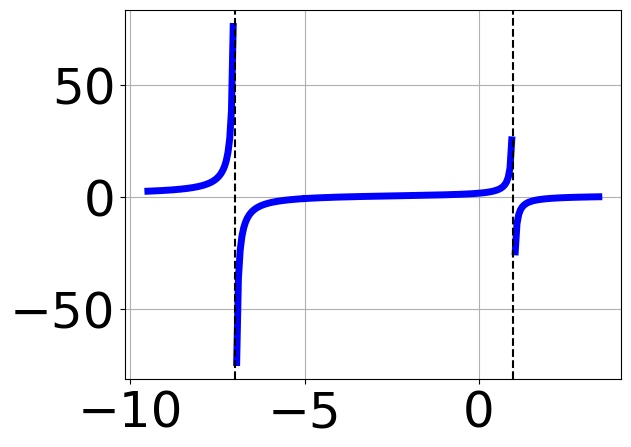
\includegraphics[width=0.5\textwidth]{../Figures/identifyGraphOfRationalFunctionB.png}
\end{center}
\begin{enumerate}[label=\Alph*.]
\item \( f(x)=\frac{x^{3} -6 x^{2} -7 x + 60}{x^{3} -11 x^{2} +23 x + 35} \)
\item \( f(x)=\frac{x^{3} -3 x^{2} -16 x + 48}{x^{3} +11 x^{2} +23 x -35} \)
\item \( f(x)=\frac{x^{3} -6 x^{2} -7 x + 60}{x^{3} -11 x^{2} +23 x + 35} \)
\item \( f(x)=\frac{x^{3} +6 x^{2} -7 x -60}{x^{3} +11 x^{2} +23 x -35} \)
\item \( \text{None of the above are possible equations for the graph.} \)

\end{enumerate} }
\litem{
Determine the horizontal and/or oblique asymptotes in the rational function below.\[ f(x) = \frac{9x^{3} -15 x^{2} -26 x + 40}{3x^{2} +8 x -16} \]\begin{enumerate}[label=\Alph*.]
\item \( \text{Horizontal Asymptote of } y = 3.0 \text{ and Oblique Asymptote of } y = 3x -13 \)
\item \( \text{Horizontal Asymptote of } y = -4.0 \text{ and Oblique Asymptote of } y = 3x -13 \)
\item \( \text{Horizontal Asymptote of } y = 3.0  \)
\item \( \text{Horizontal Asymptote at } y = -4.0 \)
\item \( \text{Oblique Asymptote of } y = 3x -13. \)

\end{enumerate} }
\litem{
Determine the horizontal and/or oblique asymptotes in the rational function below.\[ f(x) = \frac{10x^{3} +19 x^{2} -94 x -40}{-4x^{3} +24 x^{2} +46 x -40} \]\begin{enumerate}[label=\Alph*.]
\item \( \text{None of the above} \)
\item \( \text{Vertical Asymptote of } y = 1.000  \)
\item \( \text{Vertical Asymptote of } y = -4  \)
\item \( \text{Horizontal Asymptote of } y = -2.500  \)
\item \( \text{Horizontal Asymptote of } y = 0  \)

\end{enumerate} }
\litem{
Determine the vertical asymptotes and holes in the rational function below.\[ f(x) = \frac{12x^{3} +79 x^{2} +144 x + 80}{6x^{2} -7 x -20} \]\begin{enumerate}[label=\Alph*.]
\item \( \text{Vertical Asymptote of } x = 2.5 \text{ and hole at } x = -1.333 \)
\item \( \text{Holes at } x = 2.5 \text{ and } x = -1.333 \text{ with no vertical asymptotes.} \)
\item \( \text{Vertical Asymptotes of } x = 2.5 \text{ and } x = -1.333 \text{ with no holes.} \)
\item \( \text{Vertical Asymptote of } x = 2.0 \text{ and hole at } x = -1.333 \)
\item \( \text{Vertical Asymptotes of } x = 2.5 \text{ and } x = -1.25 \text{ with a hole at } x = -1.333 \)

\end{enumerate} }
\litem{
Which of the following functions \textit{could} be the graph below?
\begin{center}
    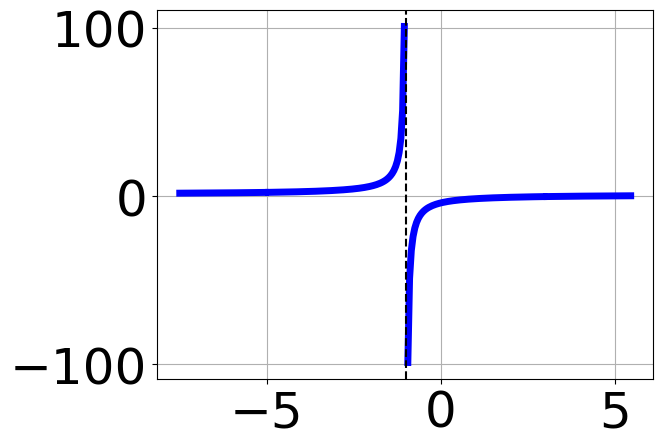
\includegraphics[width=0.5\textwidth]{../Figures/identifyGraphOfRationalFunctionCopyB.png}
\end{center}
\begin{enumerate}[label=\Alph*.]
\item \( f(x)=\frac{x^{3} +2 x^{2} -23 x -60}{x^{3} -3 x^{2} -13 x + 15} \)
\item \( f(x)=\frac{x^{3} -2 x^{2} -23 x + 60}{x^{3} +3 x^{2} -13 x -15} \)
\item \( f(x)=\frac{x^{3} +2 x^{2} -23 x -60}{x^{3} -3 x^{2} -13 x + 15} \)
\item \( f(x)=\frac{x^{3} -7 x^{2} +2 x + 40}{x^{3} +3 x^{2} -13 x -15} \)
\item \( \text{None of the above are possible equations for the graph.} \)

\end{enumerate} }
\litem{
Determine the horizontal and/or oblique asymptotes in the rational function below.\[ f(x) = \frac{12x^{3} -49 x^{2} -2 x + 24}{4x^{2} -23 x + 15} \]\begin{enumerate}[label=\Alph*.]
\item \( \text{Horizontal Asymptote of } y = 3.0 \text{ and Oblique Asymptote of } y = 3x + 5 \)
\item \( \text{Oblique Asymptote of } y = 3x + 5. \)
\item \( \text{Horizontal Asymptote of } y = 5.0 \text{ and Oblique Asymptote of } y = 3x + 5 \)
\item \( \text{Horizontal Asymptote at } y = 5.0 \)
\item \( \text{Horizontal Asymptote of } y = 3.0  \)

\end{enumerate} }
\litem{
Determine the vertical asymptotes and holes in the rational function below.\[ f(x) = \frac{4x^{3} -12 x^{2} -25 x + 75}{4x^{2} -4 x -15} \]\begin{enumerate}[label=\Alph*.]
\item \( \text{Vertical Asymptotes of } x = -1.5 \text{ and } x = 2.5 \text{ with no holes.} \)
\item \( \text{Vertical Asymptotes of } x = -1.5 \text{ and } x = -2.5 \text{ with a hole at } x = 2.5 \)
\item \( \text{Vertical Asymptote of } x = -1.5 \text{ and hole at } x = 2.5 \)
\item \( \text{Vertical Asymptote of } x = 1.0 \text{ and hole at } x = 2.5 \)
\item \( \text{Holes at } x = -1.5 \text{ and } x = 2.5 \text{ with no vertical asymptotes.} \)

\end{enumerate} }
\end{enumerate}

\end{document}